\documentclass[11pt,a4paper]{article}
\usepackage[T1]{fontenc}
\usepackage{lmodern,amsmath,amssymb,geometry,booktabs,parskip,xcolor,graphicx,hyperref}
\geometry{margin=2.3cm}
\hypersetup{colorlinks=true,linkcolor=blue!60!black,urlcolor=blue!60!black}
\graphicspath{{../simulation/figures/}}
% Written by simulation/make_numbers.py; do not edit.
\newcommand{\TAFive}{1.4\times10^{12}}
\newcommand{\TAsingleFive}{1.2\times10^{11}}
\newcommand{\QAFive}{161}
\newcommand{\TBFive}{1.5\times10^{10}}
\newcommand{\QBFive}{137}
\newcommand{\TAOne}{1.1\times10^{14}}
\newcommand{\TAsingleOne}{1.0\times10^{13}}
\newcommand{\QAOne}{186}
\newcommand{\TBOne}{2.2\times10^{12}}
\newcommand{\QBOne}{160}
\newcommand{\TATenth}{1.9\times10^{17}}
\newcommand{\TAsingleTenth}{1.8\times10^{16}}
\newcommand{\QATenth}{231}
\newcommand{\TBTenth}{8.6\times10^{15}}
\newcommand{\QBTenth}{187}
\newcommand{\RatioAB}{52}
\newcommand{\RatioABSingle}{4.7}
\newcommand{\StepsA}{3512}
\newcommand{\StepsB}{1812}
\newcommand{\ReadoutRuns}{7.9\times10^{5}}
\newcommand{\RunsBOne}{4.6\times10^{5}}
\newcommand{\OracleShareA}{83}
\newcommand{\PrepShareA}{0.5}
\newcommand{\SerialDaysB}{25}
\newcommand{\SerialYearsA}{3.5}
\newcommand{\OracleMin}{73}
\newcommand{\OracleMax}{85}
\newcommand{\KappaB}{3.88}
\newcommand{\TableA}{%
$\nu$ & 8 & 16 & 8\\
grid $N\times N$; $\Delta x$ & $32^2$; 1.000 & $64^2$; 0.667 & $256^2$; 0.121\\
readout span $h$ & 4 & 8 & 16\\
$p$-profile; $\eta_{\max}$; $n_p$ & $g_1$; 10; 9 & $g_1$; 20; 12 & $g_2$; 20; 15\\
grid error charged (measured) & $1.4\times10^{-2}$ ($6.9\times10^{-3}$) & $2.9\times10^{-3}$ ($1.7\times10^{-3}$) & $3.8\times10^{-4}$ ($1.2\times10^{-4}$)\\
LCU normalisation $\alpha$ & 45 & 155 & 2190\\
$P_{\rm succ}$ & 0.41 & 0.35 & 0.16\\
walk steps per run (standard QSP) & 641 (1228) & 3512 (6952) & 44907 (89724)\\
T per walk step (potential oracle) & 2925 (2420) & 3635 (3028) & 5200 (4428)\\
T per coherent run & $1.9\times10^{6}$ & $1.3\times10^{7}$ & $2.3\times10^{8}$\\
$\log_2M_j$, four amplitudes & 14, 12, 13, 12 & 17, 16, 17, 16 & 24, 22, 23, 23\\
coherent runs per estimate set & $6.6\times10^{4}$ & $7.9\times10^{5}$ & $7.5\times10^{7}$\\
total T, one estimate set & $1.2\times10^{11}$ & $1.0\times10^{13}$ & $1.8\times10^{16}$\\
\textbf{total T, median of 11} & $\mathbf{1.4\times10^{12}}$ & $\mathbf{1.1\times10^{14}}$ & $\mathbf{1.9\times10^{17}}$\\
\textbf{logical qubits} & \textbf{161} & \textbf{186} & \textbf{231}\\}
\newcommand{\TableB}{%
grid $N\times N$; half-width $L/\sqrt\nu$ & $32^2$; 5 & $64^2$; 5.5 & $128^2$; 6\\
$p$-profile; $\eta_{\max}$; $n_p$ & $g_{1/2}$; 5; 8 & $g_{1/2}$; 10; 10 & $g_{1/2}$; 40; 14\\
systematic error $r$ & $1.3\times10^{-2}$ & $2.2\times10^{-3}$ & $4.8\times10^{-4}$\\
LCU normalisation $\alpha$ & 51 & 148 & 470\\
$P_{\rm succ}$ & 0.65 & 0.56 & 0.43\\
walk steps per run & 428 & 1812 & 19672\\
T per walk step (potential oracle) & 1982 (1444) & 2541 (1920) & 3193 (2460)\\
T per coherent run & $8.6\times10^{5}$ & $4.7\times10^{6}$ & $6.3\times10^{7}$\\
accepted samples & $1.1\times10^{4}$ & $2.6\times10^{5}$ & $5.9\times10^{7}$\\
coherent runs & $1.8\times10^{4}$ & $4.6\times10^{5}$ & $1.4\times10^{8}$\\
\textbf{total T, 95\% target} & $\mathbf{1.5\times10^{10}}$ & $\mathbf{2.2\times10^{12}}$ & $\mathbf{8.6\times10^{15}}$\\
\textbf{logical qubits} & \textbf{137} & \textbf{160} & \textbf{187}\\}
\newcommand{\TableQ}{%
A, 5\% & 10 & 9 & 17 & 1 & 95 & 28 & 1 & 161\\
A, 1\% & 12 & 12 & 20 & 1 & 107 & 33 & 1 & 186\\
A, 0.1\% & 16 & 15 & 24 & 1 & 131 & 43 & 1 & 231\\
B, 5\% & 10 & 8 & 15 & 1 & 71 & 32 & 0 & 137\\
B, 1\% & 12 & 10 & 17 & 1 & 83 & 37 & 0 & 160\\
B, 0.1\% & 14 & 14 & 19 & 1 & 95 & 44 & 0 & 187\\}
\newcommand{\TableE}{%
5\% & $2.1\times10^{-3}$ ($4.4\times10^{-3}$) & $6.5\times10^{-3}$ & $7.6\times10^{-3}$ & 100.0 & 99.9 & 95.0 & 99.7 & 100.0\\
1\% & $7.6\times10^{-5}$ ($5.8\times10^{-4}$) & $1.8\times10^{-3}$ & $3.5\times10^{-3}$ & 100.0 & 99.6 & 90.5 & 99.0 & 99.8\\
0.1\% & $4.0\times10^{-6}$ ($3.7\times10^{-5}$) & $1.2\times10^{-4}$ & $1.5\times10^{-4}$ & 100.0 & 99.9 & 96.1 & 99.7 & 100.0\\}
\newcommand{\TableG}{%
0.2 & $8.8\times10^{-2}$ & $2.7\times10^{-2}$ & $7.0\times10^{-3}$ & $1.8\times10^{-3}$ & $2.5\times10^{-15}$\\
0.5 & $1.8\times10^{-2}$ & $4.6\times10^{-3}$ & $1.2\times10^{-3}$ & $2.9\times10^{-4}$ & $4.3\times10^{-8}$\\
1 & $2.8\times10^{-3}$ & $6.2\times10^{-4}$ & $1.5\times10^{-4}$ & $4.0\times10^{-5}$ & $1.2\times10^{-5}$\\
2 & $6.3\times10^{-3}$ & $1.4\times10^{-3}$ & $3.4\times10^{-4}$ & $8.3\times10^{-5}$ & $2.1\times10^{-4}$\\
4 & $9.8\times10^{-3}$ & $2.0\times10^{-3}$ & $4.7\times10^{-4}$ & $1.1\times10^{-4}$ & $8.9\times10^{-4}$\\
8 & $9.1\times10^{-3}$ & $2.3\times10^{-3}$ & $5.7\times10^{-4}$ & $1.3\times10^{-4}$ & $1.8\times10^{-3}$\\
16 & $8.7\times10^{-3}$ & $2.2\times10^{-3}$ & $5.4\times10^{-4}$ & $1.2\times10^{-4}$ & $2.5\times10^{-3}$\\}
\newcommand{\TableP}{%
5 (9) & $1.3\times10^{-1}$ (0.85) & $7.5\times10^{-2}$ (0.75) & $3.6\times10^{-1}$ (0.49) & $4.7\times10^{-2}$ (0.24)\\
10 (10) & $5.9\times10^{-3}$ (0.60) & $7.7\times10^{-3}$ (0.55) & $2.2\times10^{-3}$ (0.40) & $4.9\times10^{-4}$ (0.18)\\
20 (11) & $2.3\times10^{-3}$ (0.53) & $1.1\times10^{-3}$ (0.47) & $1.0\times10^{-4}$ (0.35) & $1.1\times10^{-5}$ (0.16)\\
40 (12) & $8.0\times10^{-4}$ (0.49) & $1.2\times10^{-5}$ (0.43) & $1.5\times10^{-6}$ (0.32) & $4.8\times10^{-7}$ (0.15)\\}
\newcommand{\TableC}{%
2; $32^2$; 1 & $6.3\times10^{-3}$ & $6.4\times10^{-3}$ & $2.1\times10^{-2}$\\
2; $32^2$; 2 & $5.7\times10^{-3}$ & $5.7\times10^{-3}$ & $2.2\times10^{-2}$\\
2; $32^2$; 4 & $3.2\times10^{-3}$ & $3.2\times10^{-3}$ & $2.5\times10^{-2}$\\
2; $32^2$; 8 & $9.4\times10^{-3}$ & $9.3\times10^{-3}$ & $3.6\times10^{-2}$\\
16; $64^2$; 1 & $2.2\times10^{-3}$ & $2.2\times10^{-3}$ & $2.5\times10^{-3}$\\
16; $64^2$; 2 & $2.2\times10^{-3}$ & $2.1\times10^{-3}$ & $2.5\times10^{-3}$\\
16; $64^2$; 4 & $2.1\times10^{-3}$ & $2.1\times10^{-3}$ & $2.6\times10^{-3}$\\
16; $64^2$; 8 & $1.7\times10^{-3}$ & $1.7\times10^{-3}$ & $2.9\times10^{-3}$\\
16; $64^2$; 16 & $2.7\times10^{-4}$ & $4.8\times10^{-4}$ & $4.2\times10^{-3}$\\}
\newcommand{\CfCount}{93}
\newcommand{\BKZero}{6.41\times10^{-2}}
\newcommand{\BKOne}{1.41\times10^{-2}}
\newcommand{\BKTwo}{2.77\times10^{-3}}
\newcommand{\TableT}{%
0.5 & $5.6\times10^{-3}$ ($1.6\times10^{-2}$) & $8.5\times10^{-5}$ ($8.8\times10^{-4}$) & $1.6\times10^{-6}$ ($4.3\times10^{-5}$)\\
0.4 & $3.6\times10^{-3}$ ($1.0\times10^{-2}$) & $3.5\times10^{-5}$ ($3.6\times10^{-4}$) & $4.2\times10^{-7}$ ($1.1\times10^{-5}$)\\
0.3 & $2.1\times10^{-3}$ ($5.8\times10^{-3}$) & $1.1\times10^{-5}$ ($1.1\times10^{-4}$) & $7.7\times10^{-8}$ ($2.0\times10^{-6}$)\\
0.2 & $9.1\times10^{-4}$ ($2.6\times10^{-3}$) & $2.3\times10^{-6}$ ($2.3\times10^{-5}$) & $6.9\times10^{-9}$ ($1.8\times10^{-7}$)\\
0.15 & $5.1\times10^{-4}$ ($1.4\times10^{-3}$) & $7.2\times10^{-7}$ ($7.1\times10^{-6}$) & $1.2\times10^{-9}$ ($3.2\times10^{-8}$)\\}
\newcommand{\OrderT}{2.00, 3.99, 5.98}
\newcommand{\TableD}{%
5\% & 8; $32^2$; 4 & $6.9\times10^{-3}$ & $1.4\times10^{-2}$ & $1.1\times10^{-4}$ & $1.1\times10^{-4}$ & $7.8\times10^{-3}$\\
1\% & 16; $64^2$; 8 & $1.7\times10^{-3}$ & $2.9\times10^{-3}$ & $1.3\times10^{-6}$ & $1.3\times10^{-4}$ & $2.7\times10^{-3}$\\
0.1\% & 8; $256^2$; 16 & $1.2\times10^{-4}$ & $1.8\times10^{-4}$ & $4.5\times10^{-10}$ & $3.4\times10^{-5}$ & $3.8\times10^{-4}$\\}
\newcommand{\GridEstimateCount}{91}
\newcommand{\GridEstimateTotal}{93}
\newcommand{\GridEstimateMedian}{3.2}
\newcommand{\TableS}{%
0; 1 & $8.3\times10^{13}$ & 170 & 8; $64^2$ & $1.4\times10^{12}$ & 147 & 0.56 & 98.7\\
0.2; 1 & $1.1\times10^{14}$ & 185 & 16; $64^2$ & $2.5\times10^{12}$ & 159 & 0.59 & 99.8\\
0.4; 1 & $1.1\times10^{14}$ & 186 & 16; $64^2$ & $2.2\times10^{12}$ & 160 & 0.56 & 99.0\\
0.6; 1 & $6.9\times10^{13}$ & 184 & 4; $64^2$ & $2.1\times10^{12}$ & 162 & 0.60 & 99.1\\
0.8; 1 & $9.1\times10^{13}$ & 186 & 8; $64^2$ & $3.5\times10^{12}$ & 161 & 0.53 & 99.7\\
0.4; 0.25 & $1.0\times10^{14}$ & 183 & 8; $64^2$ & $2.2\times10^{12}$ & 159 & 0.41 & 99.6\\
0.4; 4 & $2.1\times10^{14}$ & 189 & 16; $64^2$ & $4.5\times10^{12}$ & 160 & 0.47 & 99.5\\}
\newcommand{\SweepWithin}{98.7}
\newcommand{\SweepWithinA}{100.0}
\newcommand{\SweepAmin}{6.9\times10^{13}}
\newcommand{\SweepAmax}{2.1\times10^{14}}
\newcommand{\SweepBmin}{1.4\times10^{12}}
\newcommand{\SweepBmax}{4.5\times10^{12}}
\newcommand{\FacPlain}{0.46}
\newcommand{\FacMargin}{0.985}
\newcommand{\FacExact}{0.9999}
\newcommand{\GrowthBTotal}{11}
\newcommand{\TableM}{%
1 & $1.8\times10^{-1}$ & 0.49 & 0.49 & $6.0\times10^{4}$ & $1.6\times10^{6}$ & $6.5\times10^{5}$\\
2 & $6.9\times10^{-2}$ & 0.47 & 0.49 & $4.8\times10^{5}$ & $8.2\times10^{6}$ & $1.2\times10^{6}$\\
3 & $2.7\times10^{-2}$ & 0.45 & 0.48 & $2.6\times10^{6}$ & $2.9\times10^{7}$ & $1.8\times10^{6}$\\
4 & $1.0\times10^{-2}$ & 0.44 & 0.47 & $1.3\times10^{7}$ & $9.8\times10^{7}$ & $2.4\times10^{6}$\\
5 & $4.2\times10^{-3}$ & 0.42 & 0.47 & $5.5\times10^{7}$ & $3.1\times10^{8}$ & $3.0\times10^{6}$\\
6 & $1.7\times10^{-3}$ & 0.41 & 0.46 & $2.3\times10^{8}$ & $9.0\times10^{8}$ & $3.7\times10^{6}$\\
8 & $2.8\times10^{-4}$ & 0.39 & 0.45 & $3.8\times10^{9}$ & $7.3\times10^{9}$ & $5.3\times10^{6}$\\
10 & $4.8\times10^{-5}$ & 0.36 & 0.44 & $5.7\times10^{10}$ & $5.3\times10^{10}$ & $7.1\times10^{6}$\\}
\newcommand{\GrowthA}{4.1}
\newcommand{\CompileMin}{7}
\newcommand{\CompileMax}{7}
\newcommand{\CompileCount}{18}
\newcommand{\WindowGain}{6.8}
\newcommand{\UnsafeBench}{1.6}
\newcommand{\UnsafeMax}{1733}
\newcommand{\WeightBench}{1.1\times10^{-5}}
\newcommand{\WeightMax}{7.7\times10^{-5}}
\newcommand{\SingleMin}{90}
\newcommand{\SingleMax}{96}
\newcommand{\ThreeMin}{99.6}
\newcommand{\LowerBound}{98.1}
\newcommand{\TableN}{%
0.1; 1\% & $1.5\times10^{-1}$ & $1.6\times10^{-10}$ & $2.6\times10^{13}$ & $3.6\times10^{7}$ & $1.0\times10^{-2}$ & $16^2$; 1 & $5.1\times10^{3}$ & $3.0\times10^{10}$ & 112\\
0.1; 0.1\% & $1.3\times10^{-2}$ & $2.7\times10^{-95}$ & $2.5\times10^{98}$ & $7.7\times10^{11}$ & $2.0\times10^{-3}$ & $16^2$; 1 & $2.0\times10^{5}$ & $2.2\times10^{12}$ & 120\\
0.5; 1\% & $5.3\times10^{-2}$ & $2.5\times10^{-26}$ & $6.5\times10^{28}$ & $9.8\times10^{10}$ & $2.0\times10^{-2}$ & $16^2$; 1 & $3.7\times10^{4}$ & $2.3\times10^{11}$ & 116\\}
\newcommand{\NqDirectOne}{2.6\times10^{13}}
\newcommand{\NqRecOne}{5.1\times10^{3}}
\newcommand{\NqDirectTenth}{2.5\times10^{98}}
\newcommand{\NqRecTenth}{2.0\times10^{5}}
\newcommand{\NqRichOne}{3.6\times10^{7}}
\newcommand{\NqTOne}{3.0\times10^{10}}
\newcommand{\NqQOne}{112}
\newcommand{\NqTTenth}{2.2\times10^{12}}
\newcommand{\NqNuOne}{0.15}
\newcommand{\NqRef}{2.0}
\newcommand{\NqRefHard}{5.7}
\newcommand{\NqSlope}{0.034}
\newcommand{\NqW}{11.1}
\newcommand{\NqLower}{99.7}
\newcommand{\NqBiasZero}{7\times10^{-15}}
\newcommand{\DirA}{14}
\newcommand{\DirB}{2.9}
\newcommand{\DirQA}{16}
\newcommand{\DirQB}{11}
\newcommand{\TableX}{%
A, 5\% & 60 & (641) & $1.3\times10^{5}$ & ($6.6\times10^{4}$) & $2.6\times10^{11}$ (5.3) & 149 (161)\\
A, 1\% & 122 & (3512) & $1.6\times10^{6}$ & ($7.9\times10^{5}$) & $8.0\times10^{12}$ (14) & 170 (186)\\
A, 0.1\% & 522 & (44907) & $8.4\times10^{7}$ & ($7.5\times10^{7}$) & $2.9\times10^{15}$ (67) & 210 (231)\\
B, 5\% & 78 & (428) & $8.7\times10^{4}$ & ($1.8\times10^{4}$) & $1.4\times10^{10}$ (1.1) & 129 (137)\\
B, 1\% & 140 & (1812) & $1.9\times10^{6}$ & ($4.6\times10^{5}$) & $7.4\times10^{11}$ (2.9) & 149 (160)\\
B, 0.1\% & 266 & (19672) & $4.4\times10^{8}$ & ($1.4\times10^{8}$) & $4.2\times10^{14}$ (20) & 169 (187)\\}
\newcommand{\ZeroRiskErr}{1.4\times10^{-3}}
\newcommand{\BoundaryDiff}{1.1\times10^{-5}}

\title{\textbf{Logical qubits and T gates for two-asset optimal execution}\\[0.3em]
\large Short report on Steps 3--10}
\author{Xavier Bergeron, Quantum ETS}
\date{26 November 2026 (replaces the version of 22 November)}
\begin{document}
\maketitle
% Build from this directory. Numbers come from ../paper/generated.tex.

\section*{Answer}

Logical counts for the route Cole--Hopf, Schr\"odingerisation, qubitised simulation, readout. The error budgets use
floating-point evaluations of proved bounds; see \path{WorkPlan.tex}.

\begin{center}
\begin{tabular}{@{}lccc@{}}
\toprule
Target relative error of $\mathbf v^*(\mathbf X,0)$ & 5\% & \textbf{1\%} & 0.1\%\\
\midrule
A: amplitude estimation, qubits & \QAFive & \textbf{\QAOne} & \QATenth\\
A: T gates, one estimate set & $\TAsingleFive$ & $\TAsingleOne$ & $\TAsingleTenth$\\
A: T gates, targeting 95\% (median of 11) & $\TAFive$ & $\mathbf{\TAOne}$ & $\TATenth$\\
B: sampling, qubits & \QBFive & \textbf{\QBOne} & \QBTenth\\
B: T gates, targeting 95\% & $\TBFive$ & $\mathbf{\TBOne}$ & $\TBTenth$\\
\bottomrule
\end{tabular}
\end{center}
Readout B fits the Gaussian covariance of the solution, returns the whole feedback matrix, and does not extend to
non-quadratic problems. A direct polynomial of the same walk, without the auxiliary variable, needs \DirA{} (A) and \DirB{} (B)
times fewer T gates at 1\%. The classical Riccati solution takes less than a millisecond, so no quantum advantage is claimed.

\paragraph{Off the quadratic case.} The quadratic feedback does not depend on the artificial viscosity $\nu$, which is why large
$\nu$ can be used. With a quartic terminal penalty ($\kappa=0.1$) the bias forces $\nu\approx\NqNuOne$ at 1\%, and direct readout needs
$\NqDirectOne$ runs per estimate set. Recentring on the extremal of the quadratic model keeps the circuit and needs $\NqRecOne$ runs
($\NqTOne$ T gates in total).

\section*{What changed since 22 November}

The first version gave 172 qubits and $4.0\times10^{13}$ T gates at 1\%, and
198 and $1.4\times10^{16}$ at 0.1\%. Those figures are withdrawn:
\begin{enumerate}
\item The chosen grids met the error target only because two error terms of
opposite sign cancelled at $\mathbf X$ for the chosen readout span. The report
itself had warned against exactly this when choosing the domain. The budgets
now charge the larger of a cancellation-free estimate and a numerical
error-bound estimate. Neither numerical quantity is a validated enclosure.
\item Amplitude estimation was costed without its control qubit and with
iterate counts that were not powers of two. The comparator ancillas were
undercounted.
\item The emulation did not include the rounded potential. It now does.
\item Several statements were too strong: the boundary comparison was
quoted as exact, the wrap-around error as 4\%, the integrator as a Krylov
method, and the smooth auxiliary profile as derived here (it is a variant of
arXiv:2505.00370).
\end{enumerate}
The revision of the evening of 24 November halved the walk length (an identity term of the LCU was paid for), aligned the auxiliary grid
with the recovery window (gain \WindowGain{} in success probability), charged GQSP leakage and the acceptance fluctuation, and corrected the
statement on the growth with the number of assets.

\section*{Where the cost comes from}

\begin{enumerate}
\item Runs: $\ReadoutRuns$ per estimate set (A), $\RunsBOne$ (B) at 1\%.
\item Walk steps: about $\alpha\,\eta_{\max}T$ per run.
\item The potential oracle: \OracleMin--\OracleMax\% of a walk step.
\end{enumerate}
\begin{center}
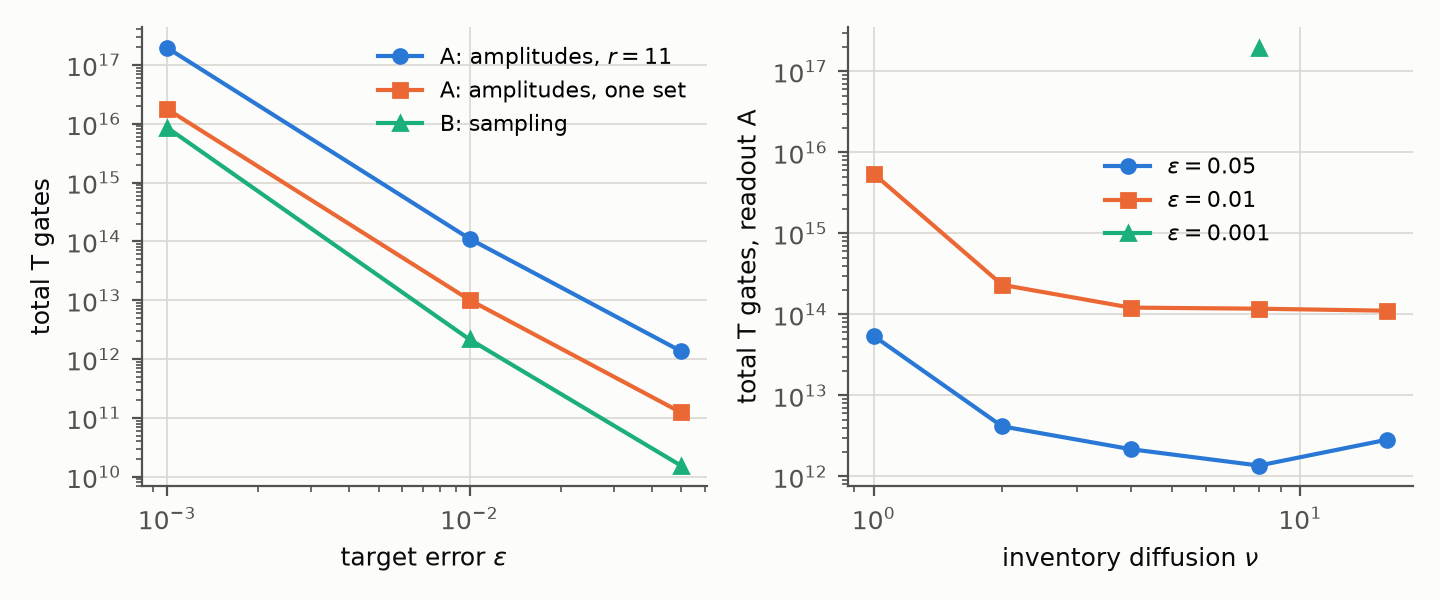
\includegraphics[width=0.95\textwidth]{tcount.png}
\end{center}
Over the $\rho$ and $\lambda$ sweeps at 1\%, A ranges over
$\SweepAmin$--$\SweepAmax$ and B over $\SweepBmin$--$\SweepBmax$ T gates. A
continuum model predicts growth of about \GrowthA{} per asset for A. The success probability of B decays by \FacMargin{} per asset
with the shifted window (\FacPlain{} without), and its runs grow by a factor \GrowthBTotal{} from 1 to 10 assets.

\section*{What is proved}

The grid error has a complete expansion with uniform remainders, for any number of assets. Its leading
part consists of a quartic and a quadratic term of strictly opposite signs, so the
radial rate error vanishes at exactly one $\nu$ (Theorem 3 of the paper). An a-posteriori bound covers the truncation to
a box. Lean~4 checks formal counterparts with the qualifications in the paper
(\path{lean/}). The charged numerical bounds use sampled floating-point
extrema, so readout-A counts are conditional. Analytic boundary and $B_2$
bounds await review. For three exploratory benchmark stencils, a rational
comparison bounds the expansion and box response; amplitude and circuit
assumptions remain unvalidated.

\section*{Evidence and limits}

Emulations of both costed pipelines (2000 trials each) meet their targets.
SELECT is compiled to gates, simulated exactly at the costed sizes, and charged at its AND count.
A small controlled walk and its inverse also pass a matrix check with ideal rotations.
GQSP truncation and gate synthesis are budgeted, not emulated. No
error-correction overhead, no simulation beyond two assets, $H=I$ and integer
$10\rho$ only. Full details: \path{paper/Paper.tex} and \path{WorkPlan.tex}.

\end{document}
